
\section{Umsetzung}
Alle gestellten Aufgaben benötigen einen OCPP Server um die OCPP Kommunikation mit der Ladesäule auswerten zu können.

Der gemeinsame Teil des Servers für alle Anwendungen ist die serverseitige OCPP Kommunikation. 
Das Verhalten auf verschiedene Nachrichten soll dabei abhörbar und leicht änderbar sein, um es für die jeweilige Anwendung anpassen zu können.

Um den Server so flexibel wie möglich zu planen, wurde von meiner Seite entschieden, ihn nach \textbf{Clean Architecture} zu implementieren.
    \subsection{OCPP Standalone Server und Testframework}
    Der OCPP Standalone Server benutzt mehrere Schnittstellen nach Außen:
    \begin{itemize}
        \item Persistenz (Datenbank und Logging)
        \item WS Server (OCPP)
        \item HTTP Server (zum Parametrieren des Verhaltens)
    \end{itemize}

    Es wird nur eine WS Server Schnittstelle vom Testframework gebraucht.
    Damit man dies mit geringsten Kosten wie möglich umsetzt, werden die Schnittstellen nach Außen mittels \textbf{Dependency Injection} benutzt. 
    
    Somit lassen viele Schnittstelle vom Server bei der Implementierung des Testframeworks gemockt bzw. 
    gefälscht werden, ohne dass man jegliches Verhalten des Programms dadurch ändern muss.

    Das Framework braucht neben dem Defaultverhalten des Programms als OCPP Server noch weitere Funktionalitäten des Testframeworks das sind 
    das Abwarten der bestimmten Events im Server um deren Inhalt auszuwerten 
    und das Ändern und das Parametrieren des Defaultverhaltens um bestimmte Situation nachbilden zu können. 
    
    Das Beobachten der Events wird mittels OOP Design Pattern \textbf{Observer} implementiert, indem man gewisse Ereignisse abonnieren kann.
    Das Ändern und das Parametrieren des Verhalten des Servers wird mittels OOP Design Pattern \textbf{Facade} und \textbf{Strategy} möglich gemacht.

    Die \textbf{Facade} ermöglicht die komplexe Architecture des Programms für den Nutzer zu verdecken um nur die wichtigen Methoden sichtbar zu machen.
    Die \textbf{Strategy} ermöglicht während das Programm läuft, das Verhalten dynamisch umzuschreiben.

    \newpage
    Beispielablauf des Frameworks:
    \begin{figure}[H]
        \centering
        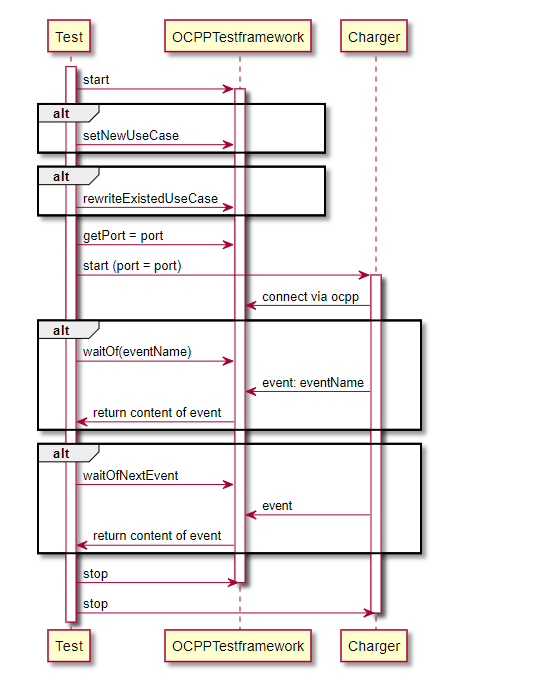
\includegraphics[width=1\textwidth]{./images/UMLFramework.png}
        \caption{Sequenzdiagramm Testframework}
        \label{fig:flow around cylinder}
        \source{Eigene Quelle}
    \end{figure}


    \subsection{ERK Automatisierungstool}
        Das Automatisierungstool sollte laut der Aufgabenstellung in einer anderen bestehenden Tool integriert werden.
        Das bereits existierte Tool ist mit Electron geschrieben, daher um das Integrationsprozess so einfach wie möglich zu machen,
        wurde von meiner Seite entschieden auch mit Electron zu arbeiten. Das ERK Tool soll 2 vorgegebenen Schnittstellen benutzen:
        \begin{itemize}
            \item Die Kommunikationsschnittstelle zu dem Autosimulator
            \item Die Kommunikationsschnittstelle zu dem Messgerät 
        \end{itemize}

        In dem bestehenden Tool wurde zur Begin der Umsetzung nur die Kommunikationsschnittstelle zum  Autosimulator implementiert,
        die Kommunikationsschnittstelle zum Messgerät wurde von dem Messgeräthersteller vorgegeben. Die Schnittstelle wurde mit einem Pythonscript implementiert.
        Damit man die Schnittstelle nicht anpassen soll um verschiedene Fehler zu vermeiden, wird das Pythonscript vom Electronprogramm mit entsprechenden Parametern gestartet, 
        und danach wird nur die Konsoleausgabe empfängt und entsprechend ausgewertet. Am Ende des Ablaufs soll ein PDF Report entstehen, das alle wichitge Informationen
        über den Testablauf beinhaltet. Neben dem Report entstehen auch 2 weitere Ausgaben:
        \begin{itemize}
            \item Logs von dem Pythonscript
            \item Alle Messdaten
        \end{itemize}

        Die Logs können später benutzt werden um die Fehler im Pythonscript zu finden und um den Testablauf später nachmachen zu können.

        Die Messdaten werden aufbewahrt um später die Richtigkeit des Reports nachweisen und mit anderen Werkzeugen überprüfen zu können.

        Benutzten Werkzeuge:
        \begin{itemize}
            \item Typescript als Programmiersprache
            \item Svelte als Frontendframework
            \item Bulma als CSS Framework
        \end{itemize}

        \newpage
        Der komplette Testablauf:
        \begin{figure}[H]
            \centering
            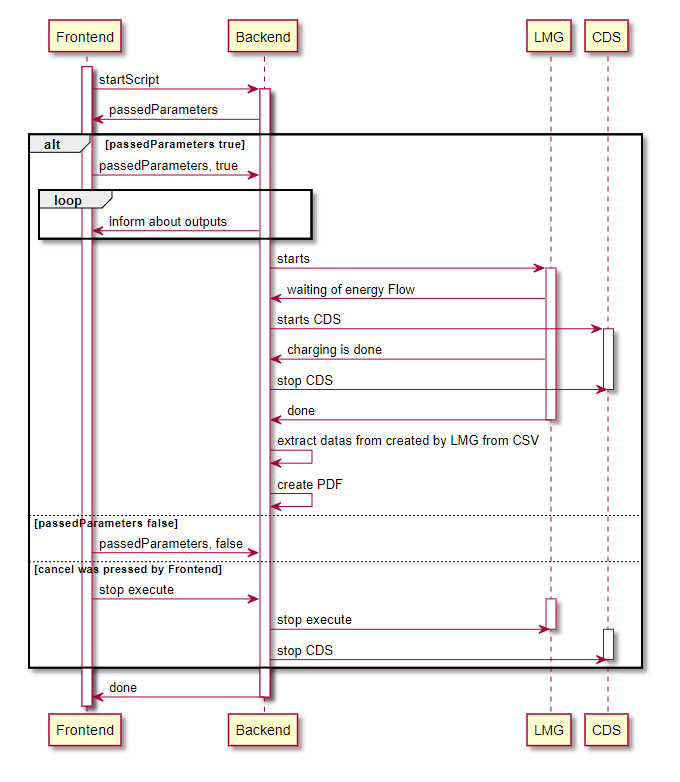
\includegraphics[width=1\textwidth]{./UML.png}
            \caption{Sequenzdiagramm ERK Tool}
            \label{fig:flow around cylinder}
            \source{Eigene Quelle}
        \end{figure}



        \newpage
        Beispiel des Reports: 
        \begin{figure}[H]
            \centering
            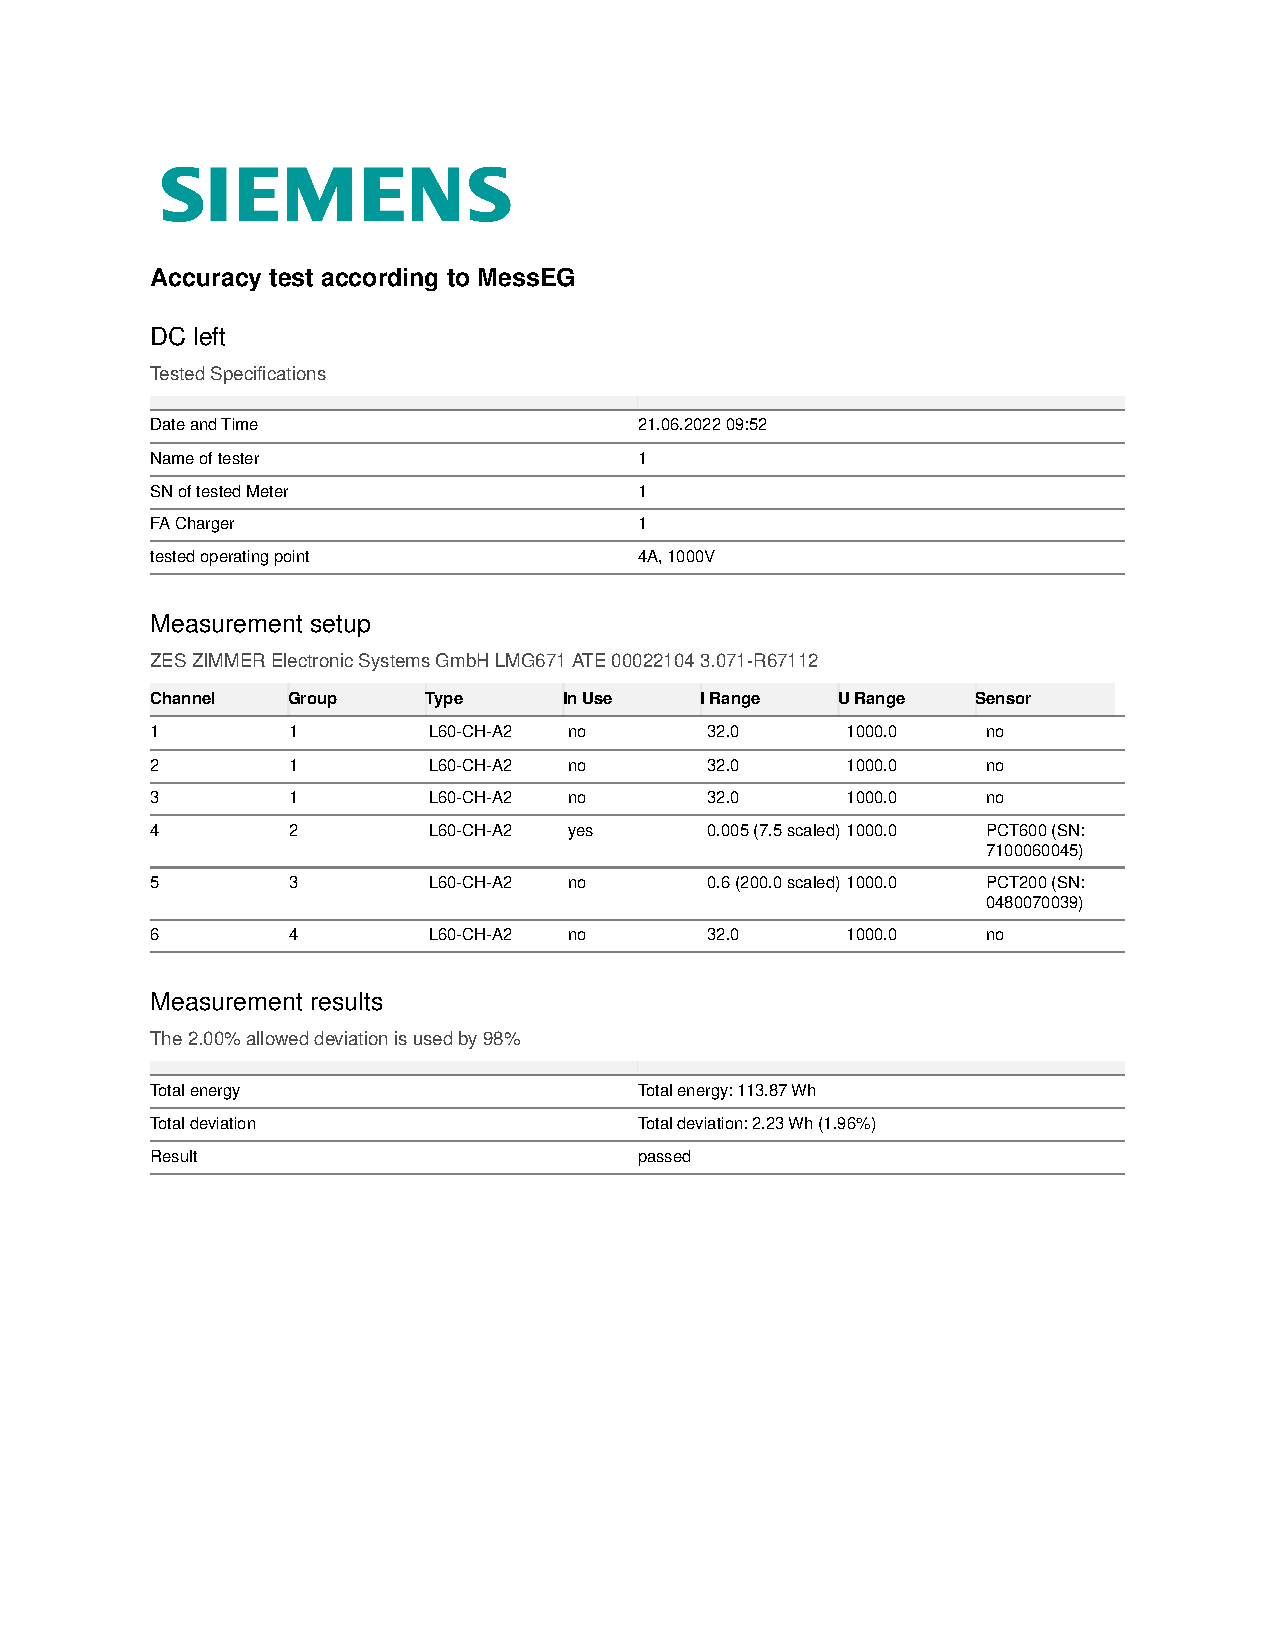
\includegraphics[width=1\textwidth]{./Report.pdf}
            \label{fig:flow around cylinder}
            \source{Eigene Quelle}
        \end{figure}